\documentclass{article}
% translate with >> pdflatex -shell-escape <file>

% This file is used as unit test for pgfplots, copyright by Christian Feuersaenger.
% 
% See
%   http://pgfplots.sourceforge.net/pgfplots.pdf
% for pgfplots.
%
% Any required input files (for <plot table> or <plot file> or the table package) can be downloaded
% at
% http://www.ctan.org/tex-archive/graphics/pgf/contrib/pgfplots/doc/latex/
% and
% http://www.ctan.org/tex-archive/graphics/pgf/contrib/pgfplots/doc/latex/plotdata/

\usepackage{pgfplots}
\pgfplotsset{compat=newest}

\pagestyle{empty}

\usepgfplotslibrary{ternary}

\begin{document}

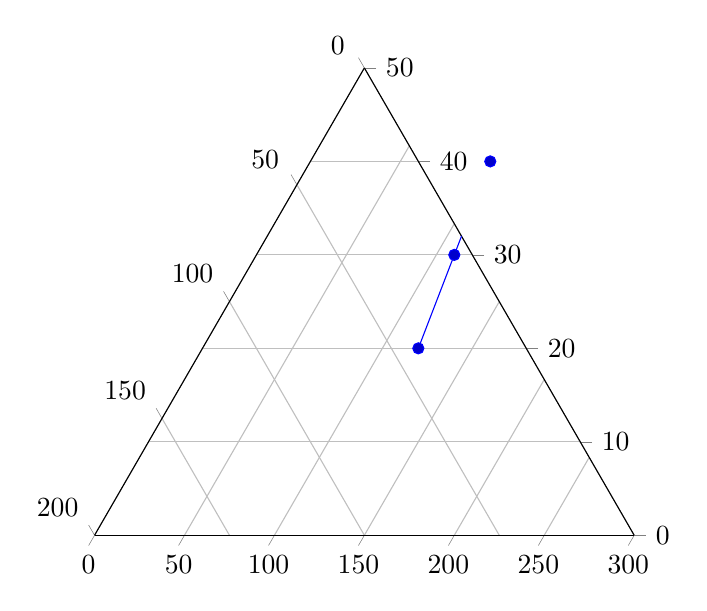
\begin{tikzpicture}
%\tracingmacros=2 \tracingcommands=2
	\begin{ternaryaxis}[
		xmin=0,xmax=50,
		ymin=0,ymax=200,
		zmin=0,zmax=300,
		ternary limits relative=false,
	]

	\addplot3 coordinates {
		(40,80,100)
		(30,50,110)
		(20,50,120)
	};
	\end{ternaryaxis}
\end{tikzpicture}
\end{document}
